\documentclass{beamer}
\beamertemplatenavigationsymbolsempty
\usepackage{amsmath, amssymb, hyperref, graphics, tikz}
%\usepackage{mathpazo, soul}



\newcommand{\C}{\mathbb{C}}
\newcommand{\Z}{\mathbb{Z}}
\newcommand{\R}{\mathbb{R}}
\newcommand{\N}{\mathbb{N}}
\DeclareMathOperator{\Real}{Re}
\DeclareMathOperator{\Imag}{Im}


\begin{document}
    \begin{frame}[plain]
        \begin{tikzpicture}[remember picture,overlay]
            \node[at=(current page.center)] {
                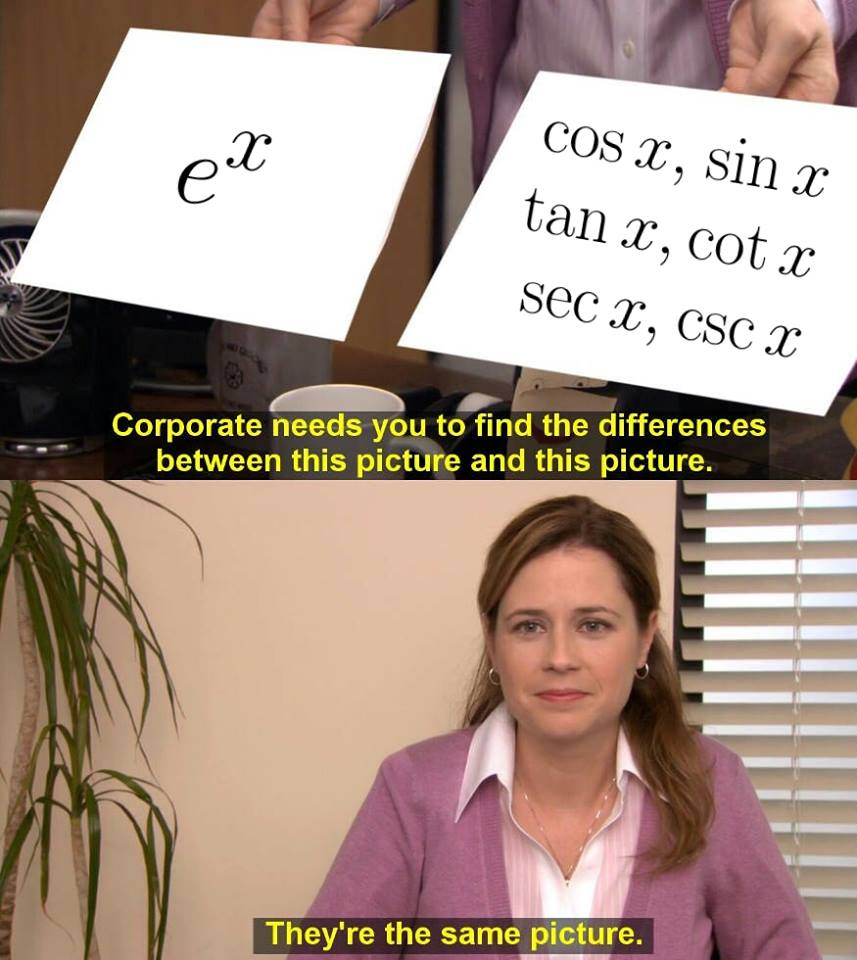
\includegraphics[keepaspectratio,
                                 width=\paperwidth,
                                 height=\paperheight]{thesame.jpg}
            };
        \end{tikzpicture}
     \end{frame}

\begin{frame}{Section 2.3 Worked examples in notes}
\begin{block}{Example 1}
Find $M$ such that 
$$\left| \frac{e^z+\cos(z)}{z+6}\right| \leq M$$
for all $z$ with $|z|=1$.
\end{block}
\begin{block}{Example 2}
Find the zeroes of $\cos(z)$
\end{block}
\end{frame}

\begin{frame}{Section 2.4: Complex Logarithm}
\begin{block}{Logs for real numbers}
For a real number $x$, $e^x>0$, and $\ln(x):(0,\infty)\to\R$ is defined to be its inverse function, i.e., $\ln(x)$ is \emph{defined} by
$$e^{\ln(x)}=x \quad\quad \ln(e^x)=x$$
\end{block}
\begin{block}{Complex case: defining $\log$}

We have defined $e^{x+iy}=e^r\left[\cos(x)+i\sin(y)\right]$ and so the codomain of the complex $\exp$ is $\C\setminus\{0\}$.  We want to define $\log$ to be the inverse function, but $\exp$ isn't one-to-one, so $\log$ won't be a function!
    \end{block}
\begin{Example}
$\log(1)$ could be $0, 2\pi i, 4\pi i, -2\pi,-56834756380\pi i\cdots$
\end{Example}

\end{frame}
\begin{frame}{Real and imaginary parts of $\log$:}
    
For $z=re^{i\theta}$, the real and imaginary parts of $\log$ are interesting.  

 $$\log(z)=\log(re^{i\theta})=\ln(r)+i\theta$$

So $\Real(\log(z))=\ln(r)=\ln(|z|)$ \emph{is} well defined.

$\Imag(\log(z))=\theta+2\pi n=\arg(z)$
\begin{Example}
Find all values of $\log(-1-i)$.

\end{Example}

\end{frame}
\begin{frame}
  
\begin{center}

\Huge

\usebeamercolor[fg]{frametitle}
Clicker Session \\
Turning Point app or \\
ttpoll.eu 

\end{center}

\end{frame}


\begin{frame}{Section 3: Simple integrals of complex valued functions}
In MAS211, you did line integrals of real functions $f(x,y)$ along a curve in the plane $\R^2$. Complex line integrals aren't any harder.

\begin{block}{Parametric curves}
IN MAS211, you parametrized curves in $\R^2$ by 
$$x=x(t)\quad y=y(t)\quad a\leq t\leq b$$
In the complex plane, we write things slightly differently, since $z=x+iy$:
$$z=z(t)=x(t)+iy(t)\quad a\leq t\leq b$$
\end{block}

\end{frame}
\begin{frame}{}

\begin{Example}[Unit circle]
In $\R^2$, we can parameterize the unit circle by
$$x(t)=\cos(t) \quad y(t)=\sin(t)\quad 0\leq t\leq 2\pi$$
In $\C$, we can write this more compactly with Euler's theorem:
$$z(t)=e^{it}=\cos(t)+i\sin(t) \quad 0\leq t\leq 2\pi$$
\end{Example}
\end{frame}
\begin{frame}{Vocabulary: Types of curves}

\begin{definition}[A curve]A \emph{curve} $\gamma$ is a continuously differentiable complex-valued function $z$ of a real variable $t$ on $[a,b]$.
\end{definition}

\begin{definition}[A path] A \emph{path} is a finite union of curves, joined successively at end points.\end{definition}

\begin{definition}[Contour] A \emph{contour} is a path whose final point is the same as the initial point.  A contour is \emph{simple} if it has no self-intersection.
\end{definition}

\begin{block}{Important examples of paths.  How to parameterize?}
\begin{itemize}
    \item $C_r(a)$ -- the circle of radius $r$ around $a$
    \item The straight line segment from $z_0$ to $z_1$
\end{itemize}
\end{block}
\end{frame}

\begin{frame}{Line integrals: Definition is chain/rule u-substitution}

\begin{definition}[3.3 in Notes; need to use, not quote]
Let $f$ be continuous on a region containing the path $\gamma$.  Let $\gamma$ be given by $z=z(t), a\leq t\leq b$.  Then 
$$\int_\gamma f(z)\text{d}z := \int_a^b f(z(t))z^\prime(t)\text{d}t$$
\end{definition}

\begin{block}{What about the fact that it's complex?}
  Just use linearity of integrals to turn it into real integrals! \\
  If $g=\Real{f}$ and $h=\Imag(f)$ then
  
$$\int_a^b f(t)\text{d}t=\int_a^bg(t)+ih(t)\text{d}t=\int_a^b g(t)\text{d}t+i\int_a^b g(t)\text{d}t$$
\end{block}
\end{frame}
\begin{frame}{Basic properties of line integrals}
\begin{block}{Basic properties -- analogous to usual integrals}
\begin{itemize}
    \item $\int_{-\gamma}f(z)\text{d}z=-\int_\gamma f(z)\text{d}z$
    \item $\int_{\gamma}(af(z)+bf(z)\text{d}z=a\int_\gamma f(z)\text{d}z+b\int_\gamma g(z)\text{d} z\quad a,b\in\C$
\item $\int_{\gamma_1+\gamma_2}f(z)\text{d}z=\int_{\gamma_1} f(z)\text{d}z+\int_{\gamma_2}f(z)\text{d}z$
\end{itemize}
 \end{block}
\begin{block}{One other fact}
  The length of curve $\gamma$, parametrized by $z:[a,b]\to \C$ is calculated similarly as

  $$\int_a^b |z^\prime(t)|\text{d}t$$
\end{block}
\end{frame}
\end{document}
